\section{迭代展开}
\label{sec:bilevel-unrolling}

隐式微分依赖“内层已经到了解点”这一前提。如果真正运行的是有限步算法，也可以直接对算法的输出求导。于是要问：怎样对$\bm{y}^{(T)}(\bm{x})$求导，这样算出的量和隐式导数有什么关系？这种做法称为\term{迭代展开}（unrolled differentiation）。

设内层的一步更新写成
\begin{equation}
 \bm{y}^{(t+1)}=\bm{\Psi}_t(\bm{y}^{(t)},\bm{x}),\qquad t=0,\ldots,T-1.
 \label{eq:bilevel-update}
\end{equation}
梯度下降取$\bm{\Psi}_t=\bm{y}-\alpha\nabla_{\bm{y}}g$，这些更新规则本身的性质在第~\ref{chap:first-order-methods}章讨论，下面只处理沿更新传播导数时新增的对象。

\subsection{完整展开}
\label{sec:bilevel-full-unroll}

\paragraph{主要思想：把算法看成复合函数}
$\bm{y}^{(T)}$是$\bm{x}$经过$T$层复合得到的函数，对它求导只需要反复使用链式法则。图~\ref{fig:bilevel-unroll-graph}是$T=2$的计算图，$\bm{x}$进入每一步更新，所以每一层都要算一次它的影响。

\begin{BookInlineFigure}
 \centering
 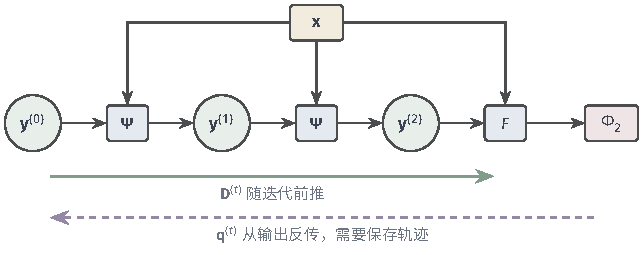
\includegraphics[width=108.9mm]{figures/05-optimization/07-multiple-criteria-and-nested-optimization/tikz/bilevel-unroll-graph/figure.pdf}
 \caption{$T=2$时的展开计算图。圆圈是内层状态，方框$\bm{\Psi}$是一步更新，$\bm{x}$进入每步更新和外层目标。绿色实线表示前向传播Jacobian矩阵$\bm{D}^{(t)}$，紫色虚线表示从外层往回传播向量$\bm{q}^{(t)}$。}
 \label{fig:bilevel-unroll-graph}
\end{BookInlineFigure}

记$\bm{D}^{(t)}\in\mathbb{R}^{d\times n}$为$\bm{y}^{(t)}$对$\bm{x}$的Jacobian矩阵，并记一步更新的两个偏导数：
\[
 \bm{A}^{(t)}=\frac{\partial\bm{\Psi}_t}{\partial\bm{y}}\in\mathbb{R}^{d\times d},\qquad
 \bm{C}^{(t)}=\frac{\partial\bm{\Psi}_t}{\partial\bm{x}}\in\mathbb{R}^{d\times n}.
\]
两者都在$(\bm{y}^{(t)},\bm{x})$处取值。对梯度下降，$\bm{A}^{(t)}=\bm{I}-\alpha\bm{H}^{(t)}$，$\bm{C}^{(t)}=-\alpha\bm{B}^{(t)}$，其中$\bm{H}^{(t)}$、$\bm{B}^{(t)}$是在当前迭代点算出的二阶导数。

对式~\eqref{eq:bilevel-update}两边关于$\bm{x}$求导。$\bm{y}^{(t)}$本身依赖$\bm{x}$，所以
\begin{equation}
 \bm{D}^{(t+1)}=\bm{A}^{(t)}\bm{D}^{(t)}+\bm{C}^{(t)}.
 \label{eq:bilevel-forward}
\end{equation}

有限步目标的梯度由链式法则得到：
\begin{equation}
 \nabla\Phi_T=\nabla_{\bm{x}}F+(\bm{D}^{(T)})^{\top}\nabla_{\bm{y}}F,
 \label{eq:bilevel-finite-gradient}
\end{equation}
其中$F$的导数在$(\bm{x},\bm{y}^{(T)})$处取值。这是精确的导数，只不过它是$\Phi_T$的导数。

\paragraph{主要思想：反向累积}
式~\eqref{eq:bilevel-forward}要带着一个$d\times n$矩阵走完全程，$n$很大时存不下。把递推展开，得到
\[
 \bm{D}^{(T)}=\sum_{t=0}^{T-1}\bm{A}^{(T-1)}\cdots\bm{A}^{(t+1)}\bm{C}^{(t)}+\bm{A}^{(T-1)}\cdots\bm{A}^{(0)}\bm{D}^{(0)}.
\]

式~\eqref{eq:bilevel-finite-gradient}只需要这个矩阵的转置与一个向量的乘积，可以从左边的向量开始依次向右乘。令$\bm{q}^{(T)}=\nabla_{\bm{y}}F$，从$t=T-1$到$0$计算
\begin{equation}
 \bm{h}\leftarrow\bm{h}+(\bm{C}^{(t)})^{\top}\bm{q}^{(t+1)},\qquad
 \bm{q}^{(t)}=(\bm{A}^{(t)})^{\top}\bm{q}^{(t+1)}.
 \label{eq:bilevel-reverse}
\end{equation}
$\bm{h}$的初值是$\nabla_{\bm{x}}F$，循环结束后再加上$(\bm{D}^{(0)})^{\top}\bm{q}^{(0)}$，结果就是$\nabla\Phi_T$。

两种顺序保存的东西不同。前向传播保存$\bm{D}^{(t)}$，不用保存轨迹。反向累积只保存向量，但$\bm{A}^{(t)}$、$\bm{C}^{(t)}$要在$\bm{y}^{(t)}$处计算，所以必须把整条轨迹保存下来，或者重新算出来。

\paragraph{计算过程}
用正则拟合例在$x=0$处计算$\Phi_3'(0)$，内层取$y^{(0)}=0$，$\alpha=1/2$。

\needspace{6\baselineskip}
\paragraph{变量}
\begin{itemize}
 \item 迭代点$y^{(t)}$，前向时的导数$D^{(t)}$，这里$d=n=1$，它们都是数。
 \item 一步更新的偏导数$A^{(t)}=1-\alpha(1+x)$，$C^{(t)}=-\alpha y^{(t)}$。
 \item 反向时的累积量$q^{(t)}$和结果$h$。
\end{itemize}

\paragraph{初始化}
初值不依赖$x$，所以$D^{(0)}=0$。例中$x=0$，于是$A^{(t)}=1/2$，$C^{(t)}=-y^{(t)}/2$。

\needspace{6\baselineskip}
\paragraph{每轮更新}
\begin{enumerate}
 \item 前向：更新$y^{(t+1)}$，并按式~\eqref{eq:bilevel-forward}更新$D^{(t+1)}$。

 例中第一轮$D^{(1)}=\frac12\cdot0-\frac12\cdot0=0$，第二轮用$y^{(1)}=3/2$，第三轮用$y^{(2)}=9/4$，各轮结果为
 \[
  y^{(1)},y^{(2)},y^{(3)}=\frac32,\ \frac94,\ \frac{21}{8};\qquad
  D^{(1)},D^{(2)},D^{(3)}=0,\ -\frac34,\ -\frac32.
 \]

 \item 走完$T$步后由式~\eqref{eq:bilevel-finite-gradient}得到梯度。

 例中$\partial_yF=y^{(3)}-1=13/8$，$\partial_xF=0$，于是
 \[
  \Phi_3'(0)=D^{(3)}\cdot\frac{13}{8}=-\frac{39}{16}.
 \]

 \item 反向：若改用反向累积，从$q^{(3)}=13/8$、$h=0$开始按式~\eqref{eq:bilevel-reverse}回算。

 例中$t=2$时$C^{(2)}=-9/8$，$t=1$时$C^{(1)}=-3/4$，$t=0$时$C^{(0)}=0$，各轮结果为
 \[
  h:\ -\frac{117}{64},\ -\frac{156}{64},\ -\frac{156}{64};\qquad
  q^{(2)},q^{(1)},q^{(0)}=\frac{13}{16},\ \frac{13}{32},\ \frac{13}{64}.
 \]
\end{enumerate}

最终$h=-156/64=-39/16$，与前向结果相同。这个数是$\Phi_3$的精确导数，而$\Phi$的导数是$-6$，两者相差很大，都是正确的导数，只是对应不同的目标。

\paragraph{初始化、动量与不可微更新}
若初值依赖$\bm{x}$，$\bm{D}^{(0)}$不为零，它的贡献必须保留。用上一轮解作热启动时，严格说初值也依赖过去的$\bm{x}$，把这一项丢掉就是在计算另一个量的导数。

算法含动量时，一步更新依赖不止一个迭代点。例如重球法的更新是
\[
 \bm{y}^{(t+1)}=\bm{y}^{(t)}-\alpha\nabla_{\bm{y}}g+\omega(\bm{y}^{(t)}-\bm{y}^{(t-1)}),
\]
要把$\bm{z}^{(t)}=(\bm{y}^{(t)},\bm{y}^{(t-1)})$作为完整状态，式~\eqref{eq:bilevel-forward}和式~\eqref{eq:bilevel-reverse}对$\bm{z}$成立。只对$\bm{y}$求导会漏掉上一步的影响。

邻近迭代的情况不同。第~\ref{chap:nonsmooth-composite-optimization}章的软阈值映射是分段光滑的，在分段的边界处没有经典导数，展开的公式只在迭代不落在边界上时才成立。

表~\ref{tab:bilevel-unroll-cost}比较两种传播顺序的代价，规模变量是内层维数$d$、外层维数$n$和步数$T$。反向累积的存储可以用\term{检查点}（checkpointing）减少：每隔$k$步保存一次状态，回算时从最近的检查点重算，$k\approx\sqrt{T}$时存储降到约$\sqrt{T}$个状态，代价是多大约一倍的计算量。

\begin{BookInlineTable}
 \centering
 \begin{tabular}{lll}
  \toprule
  做法 & 存储 & 每步主要运算\\
  \midrule
  前向传播 & $O(dn)$ & $n$次Hessian向量积\\
  反向累积 & $O(Td)$ & 一次Hessian向量积\\
  隐式微分 & $O(d)$ & 每次线性迭代一次积\\
  \bottomrule
 \end{tabular}
 \caption{三种超梯度计算的代价。存储只计迭代中保存的向量，隐式微分要求内层已解到解点附近，迭代次数由线性方程的精度决定。}
 \label{tab:bilevel-unroll-cost}
\end{BookInlineTable}

\subsection{截断展开}
\label{sec:bilevel-truncated}

保存整条轨迹太贵时，常见的做法是只反传末尾$\ell$步。这和少跑几步内层是两件不同的事。

\paragraph{两种缩短}
第一种，把内层步数从$T$减到$T'$。目标函数换成了$\Phi_{T'}$，它的导数依然精确，只是目标变了。第二种，内层仍跑满$T$步，反向只回到$t=T-\ell$，相当于在式~\eqref{eq:bilevel-reverse}中提前停止，并丢掉更早的响应。目标还是$\Phi_T$，算出的是它导数的近似。

\begin{theorem}[截断反传的误差]
\label{thm:bilevel-truncation}
设$\tilde{\bm{D}}$是把递推~\eqref{eq:bilevel-forward}中$\bm{D}^{(T-\ell)}$换成零后得到的矩阵。则
\begin{equation}
 \lVert(\bm{D}^{(T)}-\tilde{\bm{D}})^{\top}\nabla_{\bm{y}}F\rVert_2\leq
 \Bigl\lVert\prod_{t=T-\ell}^{T-1}\bm{A}^{(t)}\Bigr\rVert_2\lVert\bm{D}^{(T-\ell)}\rVert_2\lVert\nabla_{\bm{y}}F\rVert_2.
 \label{eq:bilevel-truncation}
\end{equation}
其中连乘按$t$从大到小自左向右排列。
\end{theorem}

\begin{proof}
从第$T-\ell$步开始展开递推，得到
\[
 \bm{D}^{(T)}=\sum_{t=T-\ell}^{T-1}\bm{A}^{(T-1)}\cdots\bm{A}^{(t+1)}\bm{C}^{(t)}+\bm{A}^{(T-1)}\cdots\bm{A}^{(T-\ell)}\bm{D}^{(T-\ell)}.
\]
$\tilde{\bm{D}}$恰好是右端的求和部分，差就是第二项。转置、右乘$\nabla_{\bm{y}}F$，再取范数即得。
\end{proof}

内层是收缩迭代时，连乘随$\ell$几何衰减，所以末尾的若干步已经包含了大部分信息。

\paragraph{正则拟合例中的比较}
$x=0$时$A=1/2$。取$T=20$，$y^{(t)}$已非常接近$3$，$\partial_yF\approx2$，只反传$\ell$步得到的结果约为
\[
 -6\bigl(1-2^{-\ell}\bigr).
\]
$\ell=1$时约为$-3$，$\ell=3$时约为$-5.25$。图~\ref{fig:bilevel-unroll-derivative}(b)中的绿线是这组值，黄线是真正只跑$T=\ell$步的$\Phi_\ell'(0)$，依次为$0,-15/16,-39/16$等。两者随$\ell$都趋向$-6$，黄线要慢得多，因为它不仅少反传，还因内层没跑够而用错了$y$。

\begin{BookInlineFigure}
 \centering
 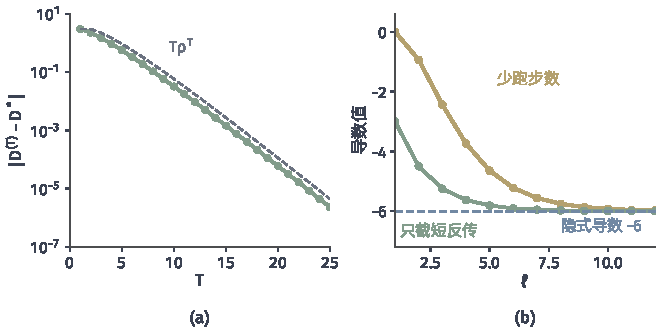
\includegraphics[width=112mm]{figures/05-optimization/07-multiple-criteria-and-nested-optimization/matplotlib/bilevel-unroll-derivative/figure.pdf}
 \caption{展开导数与隐式导数的关系，正则拟合例，$x=0$，$\alpha=1/2$。(a)绿线是导数误差$|D^{(T)}-D^\star|=3(T+1)2^{-T}$，虚线是定理~\ref{thm:bilevel-unroll-limit}型的参考界。(b)黄线是真实步数为$T=\ell$的完整展开导数，绿线是$T=20$、只反传$\ell$步的结果，蓝色虚线是隐式导数$-6$。}
 \label{fig:bilevel-unroll-derivative}
\end{BookInlineFigure}

截断后的向量一般不是$\Phi_T$的梯度，也不保证是它的下降方向。设误差向量为$\bm{e}$，真实梯度为$\bm{\gamma}$。只有在$\lVert\bm{e}\rVert_2<\lVert\bm{\gamma}\rVert_2$时才能由
\[
 \langle\bm{\gamma}+\bm{e},\bm{\gamma}\rangle\geq\lVert\bm{\gamma}\rVert_2\bigl(\lVert\bm{\gamma}\rVert_2-\lVert\bm{e}\rVert_2\bigr)>0
\]
断定它仍是下降方向。

\paragraph{与隐式微分的联系}
若内层已收敛，每一步的$\bm{A}^{(t)}$、$\bm{C}^{(t)}$都等于解点处的值$\bm{I}-\alpha\bm{H}$和$-\alpha\bm{B}$，反传$\ell$步给出
\[
 \nabla_{\bm{x}}F-\bm{B}^{\top}\Bigl[\alpha\sum_{k=0}^{\ell-1}(\bm{I}-\alpha\bm{H})^k\Bigr]\nabla_{\bm{y}}F.
\]
方括号正是式~\eqref{eq:bilevel-neumann}的前$\ell$项，所以截断反传相当于用Neumann级数的部分和代替$\bm{H}^{-1}$。

\subsection{极限关系}
\label{sec:bilevel-limit}

既然两种路线在内层收敛时形式一致，自然要问：$T\to\infty$时，展开的导数是否趋于隐式导数。答案是在收缩性等条件下成立，而只有迭代点收敛是不够的。

\begin{theorem}[展开导数的收敛]
\label{thm:bilevel-unroll-limit}
固定$\bm{x}$，内层用梯度下降，步长$\alpha\leq1/L_g$。设沿迭代路径和$\bm{y}^\star$处有$\mu\bm{I}\preceq\bm{H}\preceq L_g\bm{I}$，且存在常数$L_H,L_B$，使这些点上$\bm{H}$、$\bm{B}$关于$\bm{y}$分别$L_H$、$L_B$—Lipschitz。记
\begin{equation}
 \begin{gathered}
 \rho=1-\alpha\mu,\qquad\bm{D}^\star=-\bm{H}_\star^{-1}\bm{B}_\star,\\
 e_0=\lVert\bm{y}^{(0)}-\bm{y}^\star\rVert_2,\qquad c=\alpha(L_H\lVert\bm{D}^\star\rVert_2+L_B)e_0.
 \end{gathered}
 \label{eq:bilevel-unroll-constants}
\end{equation}
若迭代满足
\begin{equation}
 \lVert\bm{y}^{(t)}-\bm{y}^\star\rVert_2\leq\rho^te_0,
 \label{eq:bilevel-unroll-linear}
\end{equation}
则
\begin{equation}
 \lVert\bm{D}^{(T)}-\bm{D}^\star\rVert_2\leq\rho^T\lVert\bm{D}^{(0)}-\bm{D}^\star\rVert_2+cT\rho^{T-1}.
 \label{eq:bilevel-unroll-limit}
\end{equation}
\end{theorem}

\begin{proof}
先说明$\bm{D}^\star$是极限递推的不动点。把$\bm{A}_\star=\bm{I}-\alpha\bm{H}_\star$、$\bm{C}_\star=-\alpha\bm{B}_\star$代入，得到
\[
 \bm{A}_\star\bm{D}^\star+\bm{C}_\star=\bm{D}^\star-\alpha\bm{H}_\star\bm{D}^\star-\alpha\bm{B}_\star=\bm{D}^\star.
\]

记$\bm{E}^{(t)}=\bm{D}^{(t)}-\bm{D}^\star$，用递推式减去不动点方程，并在中间加减$\bm{A}^{(t)}\bm{D}^\star$，得到
\[
 \bm{E}^{(t+1)}=\bm{A}^{(t)}\bm{E}^{(t)}+(\bm{A}^{(t)}-\bm{A}_\star)\bm{D}^\star+(\bm{C}^{(t)}-\bm{C}_\star).
\]

条件$\alpha\leq1/L_g$使$\bm{A}^{(t)}$的特征值落在$[0,\rho]$，所以$\lVert\bm{A}^{(t)}\rVert_2\leq\rho$。由Lipschitz条件和式~\eqref{eq:bilevel-unroll-linear}，后两项的范数之和不超过$c\rho^t$，于是
\[
 \lVert\bm{E}^{(t+1)}\rVert_2\leq\rho\lVert\bm{E}^{(t)}\rVert_2+c\rho^t.
\]

对$T$归纳。$T=0$时式~\eqref{eq:bilevel-unroll-limit}成立。若对$T$成立，代入上式，得到
\[
 \lVert\bm{E}^{(T+1)}\rVert_2\leq\rho^{T+1}\lVert\bm{E}^{(0)}\rVert_2+cT\rho^{T}+c\rho^T=\rho^{T+1}\lVert\bm{E}^{(0)}\rVert_2+c(T+1)\rho^{T}.
\]
这就是$T+1$时的结论。
\end{proof}

收缩率$\rho$控制衰减，多出的因子$T$来自迭代点误差在每一层的累积。把结果代入式~\eqref{eq:bilevel-finite-gradient}，当$\nabla_{\bm{x}}F$、$\nabla_{\bm{y}}F$关于$\bm{y}$连续时，$\nabla\Phi_T\to\nabla\Phi$。

\paragraph{手算核对}
正则拟合例在$x=0$处，$\mu=L_g=1$，$\rho=1/2$，$L_H=0$，$L_B=1$，$e_0=3$，$c=3/2$，$\lVert D^{(0)}-D^\star\rVert=3$。式~\eqref{eq:bilevel-unroll-limit}的右端是$3\cdot2^{-T}+3T\cdot2^{-T}$。

另一方面，对式~\eqref{eq:bilevel-ridge-finite}直接求导，得到$D^{(T)}=-3+3(T+1)2^{-T}$，误差恰好等于
\[
 \lvert D^{(T)}-D^\star\rvert=3(T+1)2^{-T}.
\]
上界在这个例子里取等号。

\paragraph{点列收敛不够}
内层点列收敛这个事实本身，不足以交换求导与极限。设内层目标是$g=\frac12(y-x)^2$，$y^\star(x)=x$，某个带扰动的内层算法输出
\[
 y^{(T)}(x)=x+\frac{\sin(Tx)}{T}.
\]

对所有$x$，误差不超过$1/T$，点列一致收敛到内解。可是$\mathrm{d}y^{(T)}/\mathrm{d}x=1+\cos(Tx)$，在$x=0$处恒等于$2$，而隐式导数是$1$。误差的幅度在缩小，它的振荡频率却在增加，导数记录的恰恰是后者。定理~\ref{thm:bilevel-unroll-limit}用收缩和导数的Lipschitz条件排除了这种情形。

收缩一旦失去，结论也无从谈起。正则拟合例中$\alpha=1/2$时$q=(1-x)/2$，$x\geq3$时$\lvert q\rvert\geq1$，迭代不收敛，$\Phi_T$描述的是一个发散算法的输出。而且，固定的短展开并不自动给出真实双层目标的梯度：$T=2$时的导数$-15/16$与$-6$相差甚远。
